\documentclass[12pt]{article}
\usepackage[margin=1in]{geometry}
\usepackage{amsmath}
\usepackage{graphicx}
\usepackage{stmaryrd}

\author{Kyler Little\vspace{-0.6cm}}
\title{Homework \#2: Machine Learning\vspace{-0.3cm}}
\date{February 8, 2018\vspace{-0.7cm}}

\begin{document}
	\maketitle
	\section*{Problem \#1}
	(a) More generally, if we are learning from $\pm1$ data to predict a noisy target $P({y|\boldsymbol{x}})$ with candidate hypothesis $h$, show that the maximum likelihood method reduces to the task of finding $h$ that minimizes:
	\begin{equation*}
	E_{\text{in}}(\boldsymbol{w})= \sum_{n=1}^{N} \llbracket y_n=+1\rrbracket \ln(\frac{1}{h(\boldsymbol{x}_n)}) + \llbracket y_n=-1\rrbracket \ln \frac{1}{1-h(\boldsymbol{x}_n)}
	\end{equation*}
	Formally, we are trying to learn the target function:
	\begin{equation*}
	f(\boldsymbol{x}) = P[y=+1|\boldsymbol{x}]
	\end{equation*} 
	In non-mathematical terms, this target function represents the probability of getting $y_n=+1$ from the data ($\boldsymbol{x}_n$). The function $f$ is generated by a noisy target function, so the data doesn't give us the value of $f$ explicitly. Instead, the data is generated by a noisy target function $P(y|\boldsymbol{x})$. Our goal is to minimize the error between the classifications of actual training data and the predicted classifications from our hypothesis model $h$. We can do this by talking about the notion of likelihood. The likelihood that the target distribution $P(y|\boldsymbol{x})$ is captured by our hypothesis $h(\boldsymbol{x})$ is:
	\begin{equation*}
	P(y|\boldsymbol{x}) = 
	\begin{cases}
	h(\boldsymbol{x}) & \text{for } y=+1; \\
	1-h(\boldsymbol{x}) & \text{for } y=-1. \\
	\end{cases}
	\end{equation*}
	If we assume that the data points were independently generated (a very fair assumption to make), then we can express the probability of getting all of the $y_n$'s in the data set from their corresponding $x_n$'s as:
	\begin{equation*}
	\prod_{n=1}^{N} P(y_n|\boldsymbol{x}_n) 
	\end{equation*}
	The method of maximum likelihood method would select the hypothesis $h$ which maximizes the probability above. We can actually express this maximization problem as a minimization problem by using the properties of '$\ln$'. The natural logarithm is a monotonically increasing function, and so taking the natural logarithm of the probability above will not affect the maximization problem. By the same token, '$-\ln$' is a monotonically decreasing function, so we can take the natural logarithm of the probability above and convert the maximization problem to a minimization problem without affecting global minima of the probability distribution. Using a simple logarithm rule ($-\ln x =\ln x^{-1}$), we find:
	\begin{equation*}
	\prod_{n=1}^{N} P(y_n|\boldsymbol{x}_n) = \sum_{n=1}^{N} \ln \frac{1}{P(y_n|\boldsymbol{x}_n)}
	\end{equation*}
	Substituting in what $P(y|\boldsymbol{x})$ actually equals, we arrive at what we wanted. We now find $h$ that minimizes:
	\begin{equation*}
	E_{\text{in}}(\boldsymbol{w})= \sum_{n=1}^{N} \llbracket y_n=+1\rrbracket \ln\frac{1}{h(\boldsymbol{x}_n)} + \llbracket y_n=-1\rrbracket \ln \frac{1}{1-h(\boldsymbol{x}_n)}
	\end{equation*}
	(b) For the case $h(\boldsymbol{x}) = \theta (\boldsymbol{w}^T\boldsymbol{x})$, argue that minimizing the in-sample error in part (a) is equivalent to minimizing the one in (3.9). \\
	Substitute in $h(\boldsymbol{x}) = \theta (\boldsymbol{w}^T\boldsymbol{x}) = \frac{e^{w^T \boldsymbol{x}}}{1+e^{w^T \boldsymbol{x}}}$ to the in-sample error from part (a). This yields:
	\begin{equation*}
	E_{\text{in}}(\boldsymbol{w})= \sum_{n=1}^{N} \llbracket y_n=+1\rrbracket \ln\frac{1+e^{w^T \boldsymbol{x}}}{e^{w^T \boldsymbol{x}}} + \llbracket y_n=-1\rrbracket \ln (1+e^{w^T \boldsymbol{x}})
	\end{equation*}
	Next, use the rule $b\log(x)=\log(x^b)$ to bring the $y_n$'s inside the logarithms and $\log a + \log b = \log(ab)$ to reduce the two expression to a single expression:
	\begin{equation*}
	E_{\text{in}}(\boldsymbol{w})= \sum_{n=1}^{N} \ln (1+e^{-y_n w^T \boldsymbol{x}})
	\end{equation*}
	Multiplying by a constant factor of $1/N$ will not change the minimization problem. Thus, the argument is complete.
	\\
	\textbf{Side Note (from LFD):} \\
	For two probabilistic distributions ${p, 1-p}$ and ${q, 1-q }$ with binary outcomes, the cross-entropy (from information theory) is:
	\begin{equation*}
		p\log\frac{1}{q} + (1-p)\log\frac{1}{1-q}
	\end{equation*}
	The in-sample error in part (a) corresponds to a cross-entropy error measure on the data point $(\boldsymbol{x}_n, y_n)$, with $p=\llbracket y_n=+1\rrbracket$ and $q=h(\boldsymbol{x}_n)$.
	
	
	
	
	\section*{Problem \#2}
	Recall the objective function for linear regression can be expressed as 
	\begin{equation*}
	E(w) = \frac{1}{N} ||Xw-y||^2
	\end{equation*}
	as in Equation (3.3) of LFD. Minimizing this function with respect to $w$ leads to the optimal
	$w$ as $(X T X)^{-1} X^T y$. This solution holds only when $X^TX$ is nonsingular. To overcome this problem, the following objective function is commonly minimized instead:
	\begin{equation*}
	E_2(w) = ||Xw-y||^2 + \lambda ||w||^2
	\end{equation*}
	where $\lambda > 0$ is a user-specified parameter. Please do the following: \\
	(a) Derive the optimal $w$ that minimize $E_2(w)$.\\
	This is fairly straightforward. We differentiate $E_2(w)$, set the result to zero, and solve for $w$. The reason we can do this is because $E_2(w)$ is a convex function. This means its derivative is a monotonically increasing function, signifying that there is a unique global minimum. 
	Before differentiating, it's necessary to reduce $E_2(w)$ to an expression that is more easily differentiated. To start, we recall that $||x||=\sqrt{x^T x}$. Applying this yields:
	\begin{equation*}
	E_2(w) = \frac{1}{N}((Xw-y)^T(Xw-y)+\lambda w^T w)
	\end{equation*}
	Expanding this out yields:
	\begin{equation*}
	E_2(w) = \frac{1}{N} (w^T X^T X w-w^T X^T y-y^T Xw+y^T y + \lambda w^T w)
	\end{equation*}
	Note that $w^T X^T y=(y^T Xw)^T$, so we may combine the second and third terms, since they are identical real numbers after evaluation, resulting in $-w^T X^T y -y^T Xw=-2w^T X^T y$. Now, we simply must take the derivative of $E_2(w)$, set it to $0$, and solve for $w$. For the first term, we use the fact that $\frac{\partial(w^T Aw)}{\partial w} = (A+A^T)w$. Since $A$ is symmetric, we have that $(A+A^T)w=2Aw$. In our situation, $A$ is replaced by $X^T X$, so $\frac{\partial(w^T X^T Xw)}{\partial w} = 2X^T Xw$. For the second term, we know that $\frac{\partial(2w^T X^T y)}{\partial w} = 2X^T y$, as discussed in class. The third term disappears since it is constant with respect to $w$. The last term seems tricky at first, but an easy solution is illuminated by writing $w^T w$ as $w_1^2+\cdots+w_n^2$. Thus, $\partial (\lambda w^T w) / \partial w_i = 2\lambda w_i$. This holds $\forall i \in {1,\dots, N}$, so $\partial (\lambda w^T w) / \partial w = 2\lambda w$. As a result, we have
	\begin{equation*}
	\nabla E_2(w) = \frac{1}{N} (2X^T Xw-2X^T y + 2\lambda w)
	\end{equation*}
	Now, we set $\nabla E_2(w)$ to zero and isolate $w$.
	\begin{align*}
	0 &= \frac{1}{N} (2X^T Xw-2X^T y + 2\lambda w) \\
	0 &= X^T Xw-X^T y + \lambda w \\
	X^T y &= X^T X w + \lambda w	\\
	X^T y &= (X^T X + \lambda I)w \\
	(X^T X + \lambda I)^{-1}X^T y &=(X^T X+\lambda I)^{-1}(X^T X + \lambda I) w \\
	w&=(X^T X + \lambda I)^{-1}X^T y
	\end{align*}
	(b) Explain how this new objective function can overcome the singularity problem
	of $X^T X$. \\
	We are not necessarily guaranteed that $X^T X$ is invertible. However, we will show that $(X^T X + \lambda I)$ is always invertible. We can do this by demonstrating that it's nonsingular. In this proof, we will show that $(X^T X + \lambda I)$ is a positive definite matrix, meaning that it's nonsingular. \\
	First, write $(X^T X + \lambda I)$ as $A^T A$. It's clear that $A^T A$ is still symmetric because $X^T X$ is symmetric, and subtracting $\lambda I$ won't affect $A$'s symmetry because it only affects the diagonal of $X^T X$. Now, in order for some matrix $A$ to be positive definite, we must have that $x^T Ax >0$, $\forall x \ne 0$. Let's now prove this.
	\begin{align*}
	x^T A^T A x &> 0 \\
	(Ax)^T Ax &> 0 \\
	||Ax||^2 &> 0 \\
	\end{align*}
	Why is $||Ax||^2$ strictly greater than zero? It's obvious that $||Ax||^2$ is greater than or equal to zero because the Euclidean norm is nonnegative. However, we can guarantee that $Ax$ cannot be equal to zero because subtracting the constant $\lambda$ from the diagonal of $X^T X$ gives us the liberty to always choose $\lambda$ such that $Ax$ is nonzero.
	\\
	\section*{Problem \#3}
	In logistic regression, the objective function can be written as:
	\begin{equation*}
	E(w)=\frac{1}{N} \sum_{n=1}^{N} \ln(1+e^{-y_nw^T\boldsymbol{x}_n})
	\end{equation*}
	(a) (10 points) Compute the first-order derivative $\nabla E(w)$. You will need to provide the intermediate steps of derivation.\\
	Using the chain rule, we first note that $\frac{d(\ln \boldsymbol{x})}{d\boldsymbol{x}} = \frac{1}{\boldsymbol{x}}$. Thus, we automatically have part of the derivative as
	\begin{equation*}
	\frac{1}{N} \sum_{n=1}^{N} \frac{1}{1+e^{-y_nw^Tx_n}}
	\end{equation*}
	Next, we differentiate the argument of the natural logarithm.
	\begin{equation*}
	\frac{d(1+e^{-y_nw^Tx_n})}{dw} = -y_n \boldsymbol{x}_n e^{-y_nw^Tx_n}
	\end{equation*}
	This is easy to derive. If we write $w^T \boldsymbol{x}$ as $w_1 x_1 + \cdots + w_n x_n$, then it becomes obvious why $\partial (w^T \boldsymbol{x}) / \partial w = \boldsymbol{x}$. We are left with:
	\begin{align*}
	\nabla E(w) = -\frac{1}{N} \sum_{n=1}^{N} \frac{y_n \boldsymbol{x}_n e^{-y_nw^T \boldsymbol{x}_n}}{1+e^{-y_nw^T \boldsymbol{x}_n}}
	\end{align*}
	Now, we'd like to make the exponential in the denominator positive, so we multiply by a convenient version of the number one.
	\begin{align*}
	\nabla E(w) &= -\frac{1}{N} \sum_{n=1}^{N} \frac{y_n \boldsymbol{x}_n e^{-y_nw^T\boldsymbol{x}_n}}{1+e^{-y_nw^T\boldsymbol{x}_n}} \left( \frac{1+e^{y_n w^T \boldsymbol{x}_n}/1+e^{-y_n w^T \boldsymbol{x}_n}}{1+e^{y_n w^T \boldsymbol{x}_n}/1+e^{-y_n w^T \boldsymbol{x}_n}}\right) \\	
	\nabla E(w) &= -\frac{1}{N} \sum_{n=1}^{N} \frac{y_n \boldsymbol{x}_n e^{-y_nw^T\boldsymbol{x}_n}}{1+e^{y_nw^T\boldsymbol{x}_n}} \left( \frac{1+e^{y_n w^T \boldsymbol{x}_n}}{1+e^{-y_n w^T \boldsymbol{x}_n}} \right) \\
	\nabla E(w) &= -\frac{1}{N} \sum_{n=1}^{N} \frac{y_n \boldsymbol{x}_n e^{-y_nw^T\boldsymbol{x}_n} + y_n \boldsymbol{x}_n e^0}{1+e^{y_nw^T\boldsymbol{x}_n}} \left( \frac{1}{1+e^{-y_n w^T \boldsymbol{x}_n}} \right) \\
	\nabla E(w) &= -\frac{1}{N} \sum_{n=1}^{N} \frac{y_n \boldsymbol{x}_n (e^{-y_nw^T\boldsymbol{x}_n} + 1)}{1+e^{y_nw^T\boldsymbol{x}_n}} \left( \frac{1}{1+e^{-y_n w^T \boldsymbol{x}_n}} \right) \\
	\nabla E(w) &= -\frac{1}{N} \sum_{n=1}^{N} \frac{y_n \boldsymbol{x}_n}{1+e^{y_nw^T\boldsymbol{x}_n}} 
	\end{align*}
	This is the result obtained in the book, so we are done. \\
	(b) (10 points) Once the optimal $w$ is obtained, it will be used to make predictions as follows:
	\begin{equation*}
	\text{Predicted class of x} = 
	\begin{cases}
	1 & \text{if } \theta(w^Tx) \ge 0.5 \\
	-1 & \text{if } \theta(w^Tx) < 0.5 \\
	\end{cases}
	\end{equation*}
	where the function $\theta(z) = \frac{1}{1+e^{-z}}$ looks like \\
	\begin{figure}[h]
		\begin{center}
			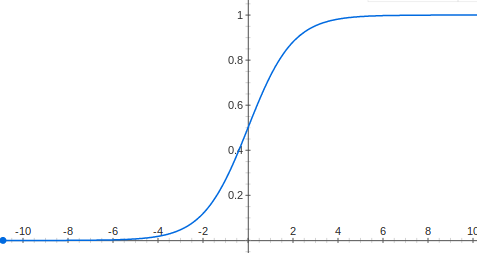
\includegraphics[width=3in]{sigmoid.png}
			\caption{A basic sigmoid curve}
			\label{fig:sigmoidEx}
		\end{center}
	\end{figure}
	\\ 
	Explain why the decision boundary of logistic regression is still linear, though the linear signal $w^Tx$ is passed through a nonlinear function $\theta$ to compute the outcome of prediction.
	Is the decision boundary still linear if the prediction rule is changed to the following? Justify briefly.
	\begin{equation*}
	\text{Predicted class of x} = 
	\begin{cases}
	1 & \text{if } \theta(w^Tx) \ge 0.9 \\
	-1 & \text{if } \theta(w^Tx) < 0.9 \\
	\end{cases}
	\end{equation*}
	The reason why the decision boundary of logistic regression is still linear is because the nonlinear function that processes the linear signal $w^T x$ is a monotonically increasing function. In other words, the output can be linearly separated because monotonically increasing/decreasing functions will never return to a value in their codomains after they have left it. Thus, even though the linear signal is passed through a nonlinear function $\theta$, the output of this nonlinear function is still linearly separable. \\
	The new decision boundary listed above is still linear because we are merely translating the boundary (which is already linear).
	\\ \\
	In light of your answers to the above two questions, what is the essential property of logistic regression that results in the linear decision boundary? \\
	The functional transformation must be monotonically increasing or decreasing. That is what allows logistic regression to retain a linear decision boundary.
	
	
	
	
	\section*{Problem \#4}
	As your final deliverable to a customer, would you use the linear model with or without the 3rd order polynomial transform? Briefly explain your reasoning. \\
	Based on my results, I would use the linear model without the 3rd order polynomial transform. The results I obtained with the 3rd order polynomial transform were not significantly better than those without the transform, as you can see in the figure below.
	\begin{figure}[h]
		\begin{center}
			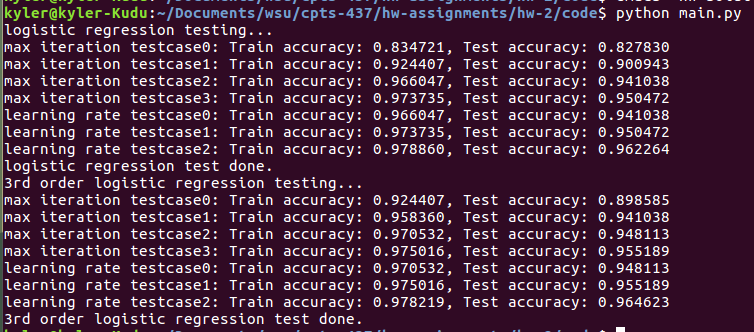
\includegraphics[width=\linewidth]{hw2_results.png}
			\caption{Logistic Regression Console Output}
			\label{fig:log_reg_results}
		\end{center}
	\end{figure}
	Although the 3rd order polynomial transform seems to do better than the unmodified linear model when the maximum iterations are low, they achieve roughly equivalent results when the maximum number of iterations is higher. Furthermore, they achieve essentially the same accuracy ratings for the same learning rates. In my opinion, the very marginal improvement in the model is not worth it due to the sacrifice in performance. The 3rd order polynomial transform adds much unnecessary overhead, and it also causes poor generalization.
	
\end{document}